%% --------------------------------------------------------------------------
%% --- Analysis scripts
%% --------------------------------------------------------------------------

\chapter{Analysis Scripts}
\label{user-analysis-scripts}

This chapter describes some tools and scripts shipped with \FramaC to help
users setup and run analyses on large code bases. These scripts can also help
dealing with unfamiliar code and automating analyses.

\section{Requirements}

These analysis scripts are chiefly based on the following tools:

\begin{description}
\item[Python]: most scripts are written using Python 3. Some scripts require
  features from specific Python versions, and perform version checks when
  starting.
\item[GNU Make]: the main workflow for analysis scripts consists in using
  GNU Make (4.0 or newer) to compute dependencies and cache intermediate
  results.
\item[Bash]: some scripts are written in Bash.
\end{description}

Besides those, a few tools are occasionally required by the scripts, such as
Perl and GNU Parallel.

\section{Usage}

Most scripts are accessible via the \texttt{frama-c-script} command, installed
along with \FramaC. Running this command without any arguments prints the list
of commands, with a brief description of each of them. Some extra scripts are
available by directly running them; in both cases, the actual scripts
themselves are installed in Frama-C's \texttt{share} directory, underneath
\texttt{analysis-scripts}.

\subsection{General Framework}

{\em Note}: while the analysis scripts are intended for usage in a wide variety
of scenarios with different plug-ins, they currently focus
on analyses with the \Value plug-in only.

The main usage mode of \texttt{analysis-scripts} consists in creating a
Makefile dedicated to the analysis of a C code base.

This Makefile has three main purposes:

\begin{enumerate}
\item To separate the main analysis steps, saving partial results and logging
  output messages;
\item To avoid recomputing unnecessary data when modifying
  analysis-specific options;
\item To document analysis options and improve replayability, e.g. when
  iteratively fine-tuning the analysis in order to improve its results.
\end{enumerate}

The intended usage is as follows:

\begin{enumerate}
\item The user identifies a C code base on which they would like to run
  Frama-C;
\item The user runs a script to interactively fill a template for
  the analysis, with the list of source files and required parameters
  (architecture, preprocessing flags, main function);
\item The user edits and runs the generated Makefile, adjusting the
  analysis as needed and re-running \texttt{fcmake}\footnote{\texttt{fcmake}
  is described in Section~\ref{sec:using-generated-makefile}.}.
\end{enumerate}

Ideally, after modifying the source code or re-parametrizing the analysis,
re-running \texttt{fcmake} should be enough to obtain a new result.

Section~\ref{sec:using-generated-makefile} details usage of the Makefile
and presents an illustrative diagram.

\subsection{Necessary Build Information}
\label{sec:necessary-build-information}

The command \texttt{frama-c-script build} can be used to generate the
Makefile from a template. To run an analysis with \Value, the following
information is necessary\footnote{If a \texttt{build\_commands.json} file is
available, \texttt{frama-c-script build} will try to fill in some of the data
automatically.}:

\begin{description}
\item[machdep]: architectural information about the system where the code will
  run: integer type sizes, compiler, OS, etc.
  See section~\ref{sec:normalize} for more details.
\item[preprocessing flags]: options given to the C preprocessor, mainly
  macros (\texttt{-D}) and include directories (\texttt{-I}).
\item[list of sources]: the actual list of source files that make a logical
  unit (e.g. a test case or a whole program), without duplicate function
  definitions.
\item[main function]: the function where the analysis will start; it is often
  \texttt{main}, but not always. ({\em Note: \FramaC itself thes not require
    a \texttt{main} function, but plug-ins such as \texttt{Eva} do}.)
\end{description}

A project without this information is incomplete; an alternative
workflow is then necessary. The next section presents some possibilities to
retrieve such information.

\subsection{Possible Workflows in the Absence of Build Information}
\label{alternative-workflows}

It is sometimes the case that the \FramaC user is not the developer of the
code under analysis, and does not have full build information about it;
or the code contains non-portable features or missing libraries which prevent
\FramaC from parsing it.
In such cases, these analysis scripts provide two alternative workflows,
depending on how one prefers to choose their source files:
{\em one at a time} or {\em all-in}, described below.

\subsubsection{One at a time}

In this workflow, the user starts from the entry point
of the analysis: typically the \texttt{main} function of a program or a test
case. Only the file defining that function is included at first. Then, using
\texttt{make-wrapper} (described in section~\ref{sec:script-descriptions}),
the user iteratively adds new sources as needed,
so that all function definitions are included.

\begin{itemize}
\item Advantages: higher code coverage; faster preprocessing/parsing; and
avoids including possibly unrelated files
(e.g. for an alternative OS/architecture).
\item Drawbacks: the iterative approach recomputes the analysis several times;
  also, it may miss files containing global initializers, which are not flagged
  as missing.
\end{itemize}

\subsubsection{All-in}

In this workflow, the user adds {\em all} source files to the analysis, and
if necessary removes some of them, e.g. when there are conflicting definitions,
such as when multiple test files define a \texttt{main} function.

\begin{itemize}
\item Advantages: optimistic approach; may not require any extra iterations, if
  everything is defined, and only once. Does not miss global initializers, and
  may find issues in code which is not reachable (e.g. syntax-related warnings).
\item Drawbacks: preprocesses and parses several files which may end up never
  being used; smaller code coverage; if parsing fails, it may be harder to
  find the cause (especially if due to unnecessary sources).
\end{itemize}

\subsection{Using a JSON Compilation Database (JCDB)}

Independently of the chosen workflow, some partial information can be retrieved
when CMake or Makefile scripts are available for compiling the sources.
They allow the production of a JSON Compilation Database
(\texttt{compile\_commands.json}, called JCDB for short; see related option
in section~\ref{sec:preprocessing}). This leads to a different workflow:

\begin{enumerate}
\item For CMake:
  \begin{itemize}
  \item Run \texttt{cmake -DCMAKE\_EXPORT\_COMPILE\_COMMANDS=1 <targets>}.
  \end{itemize}
  For Makefile:
  \begin{itemize}
  \item Install Build EAR (\url{https://github.com/rizsotto/Bear});
  \item Run \texttt{bear~make~<targets>} (instead of \texttt{make <targets>}).
  \end{itemize}
  In both cases, you will obtain a \texttt{compile\_commands.json} file.
\item Run \texttt{frama-c-script list-files}. A list of the compiled files,
  along with files defining a \texttt{main} function, will be presented.
\item Run \texttt{frama-c-script build} to create a template for
  \FramaC/\Value. It should detect the \texttt{compile\_commands.json} file
  and add the option to enable it.
\end{enumerate}

Ideally, the above approach should result in a working template. In practice,
however, the compilation database may include extraneous sources
(used to compile other files than the target object) and duplicate flags
(e.g. when compiling the same source for different binary targets or test
cases). Manual intervention may be necessary.

\section{Using the generated Makefile, via \texttt{fcmake}}
\label{sec:using-generated-makefile}

The generated Makefile can be used to run one or several analyses.
Its basic usage involving the \texttt{fcmake} alias (equivalent to
\texttt{make -C .frama-c}) is the following:

\begin{itemize}
\item \texttt{fcmake <target>.parse}: parse the sources
\item \texttt{fcmake <target>.eva}: run Eva
\item \texttt{fcmake <target>.eva.gui}: open the results in the GUI
\end{itemize}

This section details how to produce the Makefile, how to define the
\texttt{fcmake} alias, and lists other useful targets and settings.

\subsection*{Storing Frama-C files and results in \texttt{.frama-c}}

By default, the generated \texttt{GNUmakefile} is created in the (hidden)
directory \texttt{.frama-c}, which should contain all files specific to Frama-C.
This arrangement provides several benefits:

\begin{itemize}
\item Frama-C-related files do not pollute the original code; everything
  is stored in a separate directory, easily identifiable by its name;
\item Existing makefiles are not overridden by Frama-C's;
\item Having a standardized structure helps with CI integration.
\end{itemize}

However, special attention is needed due to a few consequences of this
structure:

\begin{itemize}
\item The \texttt{make} process will be run from a subdirectory of the
  current one; therefore, source and include paths must be either absolute
  or prefixed with \texttt{..};
\item In some cases, it may be necessary to add flags such as \texttt{-I ..},
  so that the preprocessor will find the required files.
\end{itemize}

\subsection*{Defining and using \texttt{fcmake}}

We recommend defining the following {\em alias} in your shell:

\begin{verbatim}
alias fcmake='make -C .frama-c'
\end{verbatim}

Running \texttt{fcmake} will have the same effect as running \texttt{make}
inside the \texttt{.frama-c} directory.

The commands in this section assume usage of the \texttt{fcmake} alias
defined above.

\subsection*{Frama-C makefile targets and variables}

The diagram in Fig.~\ref{fig:analysis-scripts} summarizes the usage of
the generated Makefile. Its targets and outputs are detailed in this section.

\begin{figure}[htbp]
  \begin{center}
    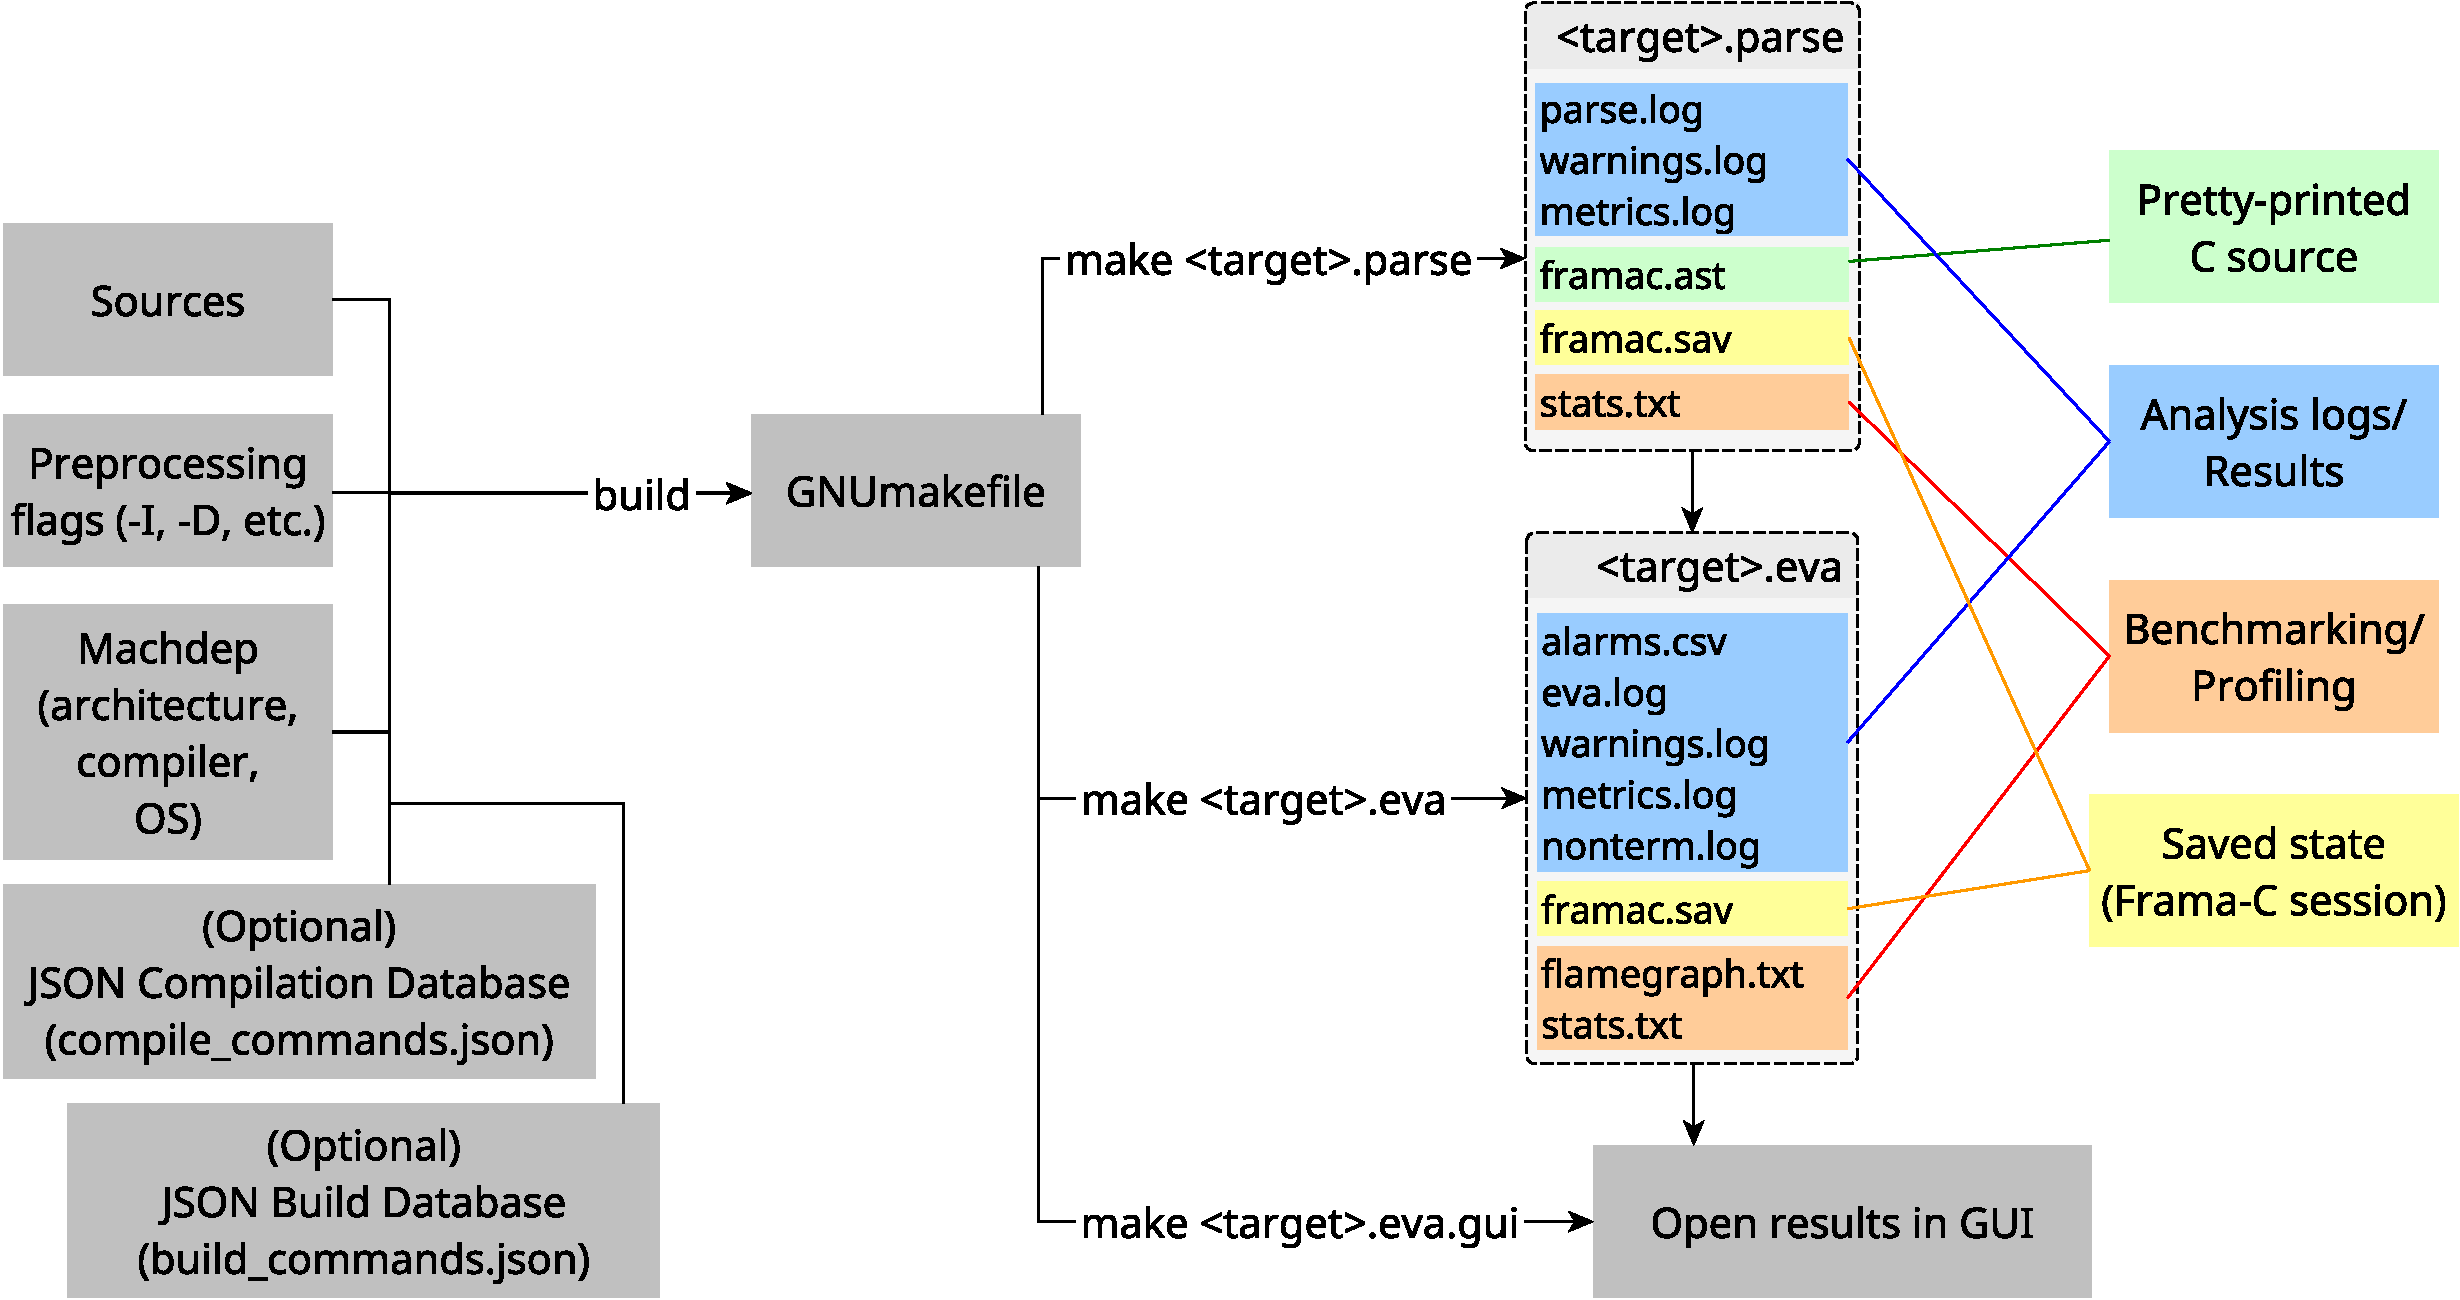
\includegraphics[width=\textwidth]{analysis-scripts.pdf}
    \caption{Overview of the {\em analysis-scripts} workflow:
      the inputs on the left produce a GNUmakefile which is then used
      for parsing, analyzing and visualizing results.}
    \label{fig:analysis-scripts}
  \end{center}
\end{figure}

Each analysis is defined in a target, written by the user as follows:

\texttt{<target>.parse: file1.c file2.c ...}

That is, the target name (chosen by the user), suffixed with \texttt{.parse},
is defined as depending on each of its source files. Changes to any of these
sources will trigger a recomputation of the AST.

Note that, since the generated makefile is inside \texttt{.frama-c}, relative
paths to source files will always begin with \texttt{../}, except for
sources located within \texttt{.frama-c}, e.g. \texttt{fc\_stubs.c}.

\begin{important}
Target names can contain hyphens and underscores, but neither slashes nor dots.
See also the {\em Technical Notes} section about some current limitations.
\end{important}

Then, for each \texttt{.parse} target, a corresponding \texttt{.eva} target
needs to be added to the \texttt{TARGETS} variable in the Makefile.
This will run \Value on the test case.

Each \texttt{.eva} target depends on its corresponding \texttt{.parse} target;
if the sources change, the analysis must take into account the new AST.

\subsection{Important Variables}

Several Makefile variables are available to customize \FramaC; the main
ones are presented below.

\begin{description}
\item[TARGETS]: as mentioned before, must contain the list of targets,
  suffixed with \texttt{.eva}.
\item[CPPFLAGS]: preprocessing options, passed to \FramaC inside option
  \texttt{-cpp-extra-args}, when parsing the sources.
\item[FCFLAGS]: extra command-line options given to \FramaC when parsing the
  sources and when running analyses. Typically, the options given to the
  \FramaC kernel.
\item[EVAFLAGS]: extra command-line options given to \Value when running
  its analyses.
\end{description}

These variables are defined globally, but they can also be customized for
each target; for instance, if a given target \texttt{t1} has a main
function \texttt{test1} and requires a global macro \texttt{-DTEST1}, but
target \texttt{t2}'s main function is \texttt{test2} and it requires
\texttt{-DTEST2}, you can locally modify \texttt{FCFLAGS} and \texttt{CPPFLAGS}
as follows:

\begin{lstlisting}
t1.parse: FCFLAGS += -main test1
t1.parse: CPPFLAGS += -DTEST1
t2.parse: FCFLAGS += -main test2
t2.parse: CPPFLAGS += -DTEST2
\end{lstlisting}

\begin{important}
\texttt{-I} flags referencing relative paths must take into account the
fact that \FramaC will be run from the \texttt{.frama-c} directory, and
therefore must include an initial ``\texttt{../}''.
\end{important}

\subsection{Predefined targets}

The predefined targets below are the {\em raison d'être} of the generated
Makefile; they speed up analyses, provide self-documentation, and enable
quick iterations during parametrization of the analysis.

\begin{description}
\item[all (default target)]: the default target simply calls
  \texttt{<target>.eva}, for each \texttt{<target>} added to variable
  \texttt{TARGETS}. Does nothing once the analysis is finished and saved.
\item[<target>.parse]: runs \FramaC on the specified target, preprocessing
  and parsing its source files. Produces a directory \texttt{<target>.parse}
  containing several logs, a pretty-printed version of the parsed code, and
  a \FramaC session file (\texttt{framac.sav}) to be loaded in the GUI or by
  other analyses. Does nothing if parsing already happened.
\item[<target>.eva]: loads the parsed result (from the \texttt{.parse} target)
  and runs the \Value plug-in, with the options given in \texttt{EVAFLAGS}.
  If the analysis succeeds, produces a directory \texttt{<target>.eva} with the
  analysis results and a saved session file.
  If the analysis fails, tries to save a partial result in
  \texttt{<target>.eva.error} (when possible).
\item[<target>.eva.gui]: loads the result of the corresponding
  \texttt{<target>.eva} session and opens it in the GUI. This allows inspecting
  the results of \Value. This target always opens the GUI, even when no
  changes have happened.
\item[clean]: removes all results produced by the \texttt{.parse} and
  \texttt{.eva} targets.
\end{description}

\subsection{Adding new analyses and stages}

Besides the predefined \Value-oriented steps, you can easily add other stages
and analyses, which may or may not depend on \Value.

For instance, to add a SARIF report using the \tool{Markdown Report} plug-in,
you can simply add, before the template epilogue, the following lines, where
\texttt{target} is the name of your target:

\begin{makefilecode}
target.sarif: target.parse
	$(FRAMAC) -load $^/framac.sav -mdr-gen sarif -mdr-out $@
\end{makefilecode}

This rule will create a file \texttt{target.sarif} inside the \texttt{.frama-c}
directory. The rule will depend on the parsing of \texttt{target.parse} and
use the saved session at \texttt{target.parse/framac.sav}.

If you want the report to run after the analysis with \Value, instead, simply
replace \texttt{.parse} with \texttt{.eva}.

Then, running \texttt{fcmake target.sarif} will create or update the report,
recomputing dependencies when needed.

Adding a new stage, with a saved session that can be reused later for other
stages and analyses, requires just a few more lines, as in the following
example:

\begin{makefilecode}
target.wp: target.parse
	mkdir -p $@
	$(FRAMAC) -load $^/framac.sav -wp -save $@/framac.sav
\end{makefilecode}

In the example above, we define a new stage, \texttt{target.wp}, which depends
on the parsing stage, runs the \tool{WP} plug-in, and saves the result in a
session file. This session file can then be loaded by another stage,
or in the GUI. For instance, the \texttt{.gui} predefined target works out of
the box in this case: running \texttt{fcmake target.wp.gui} will load the saved
session in the Frama-C GUI.

\section{Script Descriptions}
\label{sec:script-descriptions}

The most useful commands are described below.
Run \texttt{frama-c-script help} for more details and optional arguments.

\begin{description}
\item[build]: creates the initial Makefile, based on a template.
  This command creates a file named \texttt{.frama-c/GNUmakefile} with some
  hardcoded sections, some sections filled in according to command-line
  options, and some sections filled automatically with build information
  (via a \texttt{build\_commands.json} file), if available.
  Once created, it enables the general workflow mentioned earlier.
\item[make-wrapper <target> <args>]: calls \texttt{make <target> <args>} with
  a special wrapper: when running \Value, upon encountering one of a few known
  error messages, suggests some actions on how to proceed.
  For instance, if a missing function definition is encountered when analyzing
  the code with \Value, the wrapper will look for its definition and, if found,
  suggest that its source code be added to the analysis. This script is meant
  to be used with the {\em one at a time} workflow described in
  section~\ref{alternative-workflows}.
\item[find-fun <fun>]: looks for possible declarations and definitions
  of function \texttt{<fun>}. Uses a heuristic that does not depend on \FramaC
  being able to parse the sources. Useful to find entry points and missing
  includes.
\end{description}

Other commands, only useful in a few cases, are described below.

\begin{description}
\item[configure <machdep>]: runs a \texttt{configure}
  script (based on Autoconf) with some settings to emulate a more portable
  system, removing optional code features that could prevent \FramaC from
  parsing the sources. Currently, it still depends partially on the host system,
  so many features are not disabled.
\item[flamegraph]: opens a {\em flamegraph}\footnote{%
  See \url{https://github.com/brendangregg/FlameGraph} for details about
  flamegraphs.} to visualize which functions take most of the time
  during analysis with \Value.
\item[summary]: for monitoring the progression of multiple analyses defined
  in a single Makefile. Presents a summary of the analyses when done. Mostly
  useful for benchmarking or when dealing with several test cases.
\end{description}

The following commands require a JSON Compilation Database.

\begin{description}
\item[list-files]: lists all files in the given JCDB.
\item[normalize-jcdb]: converts absolute paths inside a
  \texttt{compile\_commands.json} file into relative paths (w.r.t. PWD)
  when possible. Used to allow moving/versioning the directory containing
  the JCDB file.
\end{description}

Finally, there is the following script, which is {\em not} available as a
command in \texttt{frama-c-script}, since its usage scenario is very
different. It is available at\\
\texttt{\$FRAMAC\_SHARE/analysis-scripts/creduce.sh}.

\begin{description}
\item[creduce.sh]: A script to help running the C-Reduce\footnote{%
  See \url{https://embed.cs.utah.edu/creduce} for more details.} tool to minify
  C programs causing crashes in \FramaC; useful e.g. when submitting a bug
  report to \FramaC, without needing to submit potentially confidential data.
  The script contains extensive comments about its usage. It is also
  described in a post\footnote{%
    {\em Debugging Frama-C analyses: better privacy with C-Reduce},
    at \url{https://pub.frama-c.com/scripts/usability/2020/04/02/creduce.html}.}
  from the \FramaC blog.
\end{description}

To use the \texttt{creduce.sh} script, you need to have the C-Reduce tool
installed in your path or in environment variable \texttt{CREDUCE}.

\section{Practical Examples: Open Source Case Studies}

The {\em open-source-case-studies} Git repository (OSCS for short),
available at \url{https://git.frama-c.com/pub/open-source-case-studies},
contains several open-source C code bases parametrized with the help of
analysis scripts. Each case study has its own directory, with a
\texttt{.frama-c/GNUmakefile} defining one or more analysis targets.

Due to the variety of test cases, OSCS provide practical usage
examples of the \texttt{GNUmakefile} described in this chapter.
They are periodically synchronized w.r.t. the public \FramaC repository
(daily snapshots), so they may contain features not yet available in the
major \FramaC releases. A few case studies may also contain legacy features
which are no longer used; but overall, they provide useful examples and allow
the user to tweak analysis parameters to test their effects.

\section{Technical Notes}

This section lists known issues and technical details which may help users
understand some unintuitive behaviors.

\paragraph{\em Changes to header files do not trigger a new parsing/analysis.}
Currently, changes to included files (e.g. headers) are {\em not}
tracked by the generated Makefile and may require running \texttt{fcmake}
with \texttt{-B} (to force recomputation of dependencies), or running
\texttt{fcmake clean} before re-running \texttt{fcmake}.

\paragraph{\em Most scripts are heuristics-based and offer no
  correctness/completeness guarantees.} In order to handle files {\em before}
the source preparation step is complete (that is, before \FramaC is able to
parse the sources into a complete AST), most commands use scripts based on
syntactic heuristics, which were found to work well in practice but are
easily disturbed by syntactic changes (e.g. whitespaces).

\paragraph{\em Most commands are experimental.} These analysis scripts are a
recent addition and subject to changes. They are provided on a best-effort
basis.
